\chapter{Đặt vấn đề và phân tích yêu cầu}
\section{Lý do chọn đề tài}
Trong thực tế, việc nhận biết một loài hoa qua ảnh không phải lúc nào cũng dễ dàng. Có những loại hoa có màu sắc hoặc hình dạng gần giống nhau; ngược lại, ảnh của cùng một loại có thể thay đổi nhiều do góc chụp, độ sáng, kích thước và phần nền. Khi làm bài tập môn Học máy, nhóm em chọn bài toán phân loại ảnh hoa để tìm hiểu cách chuyển ảnh thành dữ liệu số và sử dụng các thuật toán đã học để dự đoán nhãn.

Đầu vào của bài toán là một bức ảnh hoa; đầu ra là mã của một trong 102 lớp. Nhóm em tập trung vào các thuật toán học máy truyền thống, cụ thể là K-NN và cây quyết định, để có thể giải thích rõ cách trích xuất đặc trưng và so sánh kết quả. Nhóm không sử dụng mạng nơ-ron tích chập hoặc mô hình học chuyển giao trong phạm vi báo cáo này.
\section{Mục tiêu và yêu cầu}
Nhóm em đặt ra các mục tiêu: tìm hiểu dữ liệu, kiểm tra các nhãn và phần chia dữ liệu; xây dựng bước tiền xử lý thống nhất; thử đặc trưng pixel, HOG, histogram màu và PCA; huấn luyện các mô hình E1–E6; so sánh bằng các chỉ số đánh giá và phân tích lỗi. Bên cạnh điểm số, nhóm cũng kiểm tra khả năng tái lập, độ ổn định qua các fold và nguy cơ ảnh trùng giữa các tập.

Yêu cầu quan trọng là không để thông tin của tập kiểm tra làm ảnh hưởng đến việc chọn mô hình. Các phép biến đổi cần học tham số như PCA phải được học từ tập huấn luyện. Tập validation dùng để lựa chọn cấu hình; tập test dùng cho đánh giá cuối theo quy trình đã thống nhất trước, không dùng để liên tục điều chỉnh mô hình.
\section{Bộ dữ liệu và phân tích khám phá}
Nhóm em sử dụng bộ dữ liệu Oxford 102 Flowers do Đại học Oxford công bố \cite{oxford,nilsback}. Bộ dữ liệu có 8.189 ảnh thuộc 102 lớp. Dữ liệu được chia theo metadata chính thức: 1.020 ảnh train, 1.020 ảnh validation và 6.149 ảnh test. Mỗi lớp có 10 ảnh trong train và 10 ảnh trong validation; số ảnh giữa các lớp trong test không bằng nhau. Nhóm giữ nguyên cách chia này thay vì tự tạo một split mới.

Tệp nhãn chính thức đánh số lớp từ 1 đến 102. Trong mã nguồn, nhóm chuyển sang 0 đến 101 để thuận tiện cho việc xử lý, sau đó cộng lại một khi hiển thị kết quả. Kiểm toán V4 ghi nhận tất cả ảnh đều giải mã được và có chế độ RGB. Chiều rộng ảnh trong dữ liệu nằm trong khoảng 500–1.024 pixel và chiều cao trong khoảng 500–1.168 pixel. Sự khác nhau về kích thước cho thấy cần có bước đưa ảnh về một kích thước thống nhất trước khi tạo vector đặc trưng.

Hình \ref{fig:phanbo} trình bày số lượng ảnh của từng lớp trên toàn bộ bộ dữ liệu. Nhóm sử dụng hình này để hiểu cấu trúc dữ liệu, không dùng biểu đồ để thay đổi split chính thức hoặc lựa chọn mẫu test.
\begin{figure}[htbp]\centering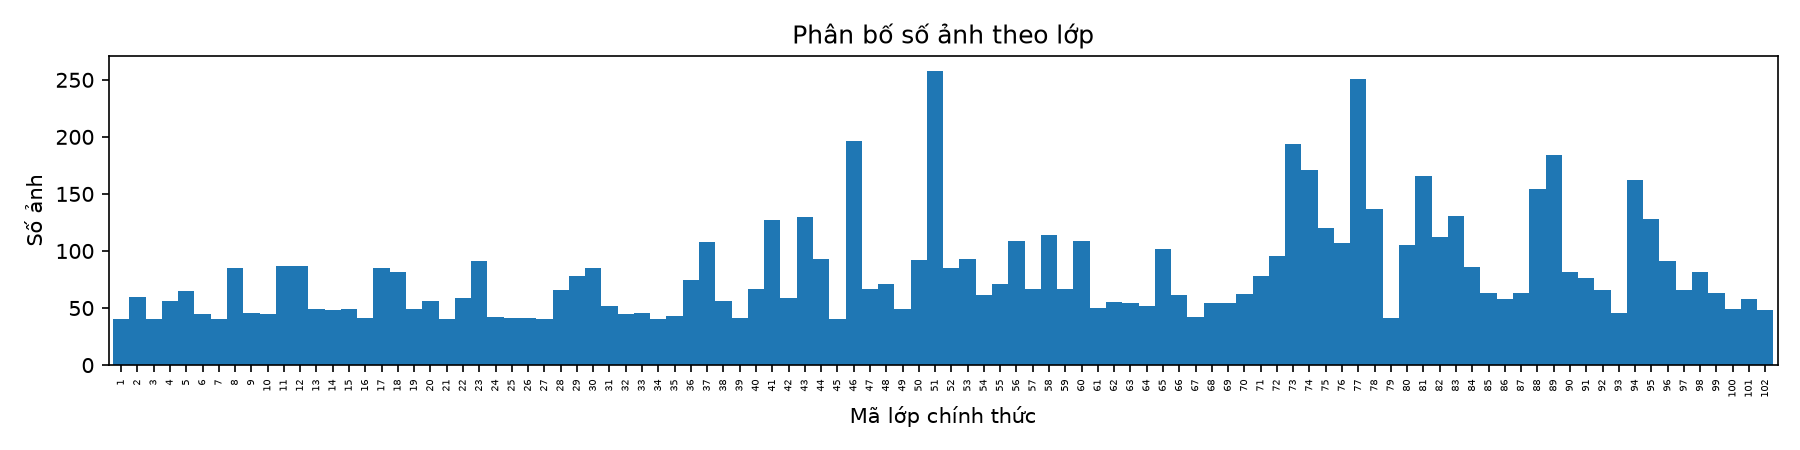
\includegraphics[width=\textwidth]{figures/phan_bo.png}\caption{Phân bố số ảnh theo mã lớp chính thức.}\label{fig:phanbo}\end{figure}
\section{Đặc điểm của bài toán phân loại nhiều lớp}
Trong bài toán này, mỗi ảnh chỉ nhận một nhãn chính thức. Tuy nhiên, việc quan sát ảnh thực tế cho thấy màu nền, lá, thân và các vật thể xung quanh cũng có thể chiếm một phần lớn diện tích ảnh. Nếu mô hình sử dụng toàn bộ ảnh, những vùng này đều góp mặt trong vector đặc trưng. Do đó, dự đoán không chỉ phụ thuộc vào phần cánh hoa mà còn có thể chịu ảnh hưởng của bố cục và màu nền.

Một khó khăn nữa là số lượng lớp lớn so với số mẫu huấn luyện. Mỗi lớp có 10 ảnh train; K-NN chỉ có thể tìm láng giềng trong số những ảnh đã biết. Nếu ảnh mới có góc chụp hoặc điều kiện sáng khác, các mẫu gần nhất trong không gian đặc trưng có thể không cùng lớp. Nhận xét này giúp giải thích vì sao cần xem cả điểm tổng hợp và lỗi của từng lớp, nhưng nó không khẳng định nguyên nhân của một ảnh dự đoán sai cụ thể.

Khi phân tích dữ liệu, nhóm em kiểm tra phân phối lớp, kích thước ảnh, tỉ lệ chiều rộng trên chiều cao, chế độ màu và ví dụ đại diện. Nhóm cũng kiểm tra những tệp không đọc được, tên tệp bất thường, nhãn ngoài khoảng và ID bị lặp giữa các split. Các bước này giúp phát hiện dữ liệu đầu vào có vấn đề trước khi huấn luyện, tránh việc chương trình âm thầm bỏ qua ảnh và tạo ra số lượng mẫu khác metadata.
\section{Yêu cầu đối với kết quả và khả năng tái lập}
Một kết quả thực nghiệm có ý nghĩa cần đi kèm cách tạo ra nó. Với mỗi cấu hình, nhóm lưu tên thí nghiệm, loại đặc trưng, tham số mô hình, thời gian fit và thời gian dự đoán. Chỉ số trên validation phải được phân biệt với chỉ số test và với các điểm trên fold của kiểm định chéo. Nhóm cũng lưu các dự đoán theo ID ảnh để có thể tính lại chỉ số hoặc kiểm tra một cặp nhầm cụ thể.

Khả năng tái lập không đồng nghĩa với việc mọi máy sẽ có thời gian chạy giống hệt nhau. Kết quả có thể chịu ảnh hưởng bởi phiên bản thư viện, kiến trúc máy và phép tính số thực. Do vậy, cùng với cấu hình và seed, nhóm ghi phiên bản môi trường và hash các artifact quan trọng. Thời gian và bộ nhớ chỉ nên được so sánh khi hiểu rõ điều kiện đo.
